
\section{Kinematik}
\subsection{Jacobi Matrix}
\textbf{Nutzen:}Bestimmen von Kräften, Drehmomenten, Geschwindigkeiten und Singularitäten am TCP.\newline
Die Jacobi-Matrix eines Roboterarms beschreibt die Abbildung von
Gelenkgeschwindigkeiten auf die Lineargeschwindigkeit des TCP
und die zeitlichen Änderungen der Orientierung des End-Effektors
bezogen auf ein Referenzkoordinatensystemk z.B. auf das
Basiskoordinatensystem O auf. \\
In der Positionsbeschreibung werden alle Parameter die einen Einfluss 
auf den Greifer haben aufgestellt und dann für die Jakobi-Matrix nach diesen Partiell abgeleitet.

\subsubsection{Vorwärtskinematik}
\vspace{-0.5cm}	
\begin{tabular}{lll}
    \textbf{Geg}&Gelenkkoordinaten und Geschwindigkeiten&$q,\; \dot{q}$\\
    &Vektor der Gelenkkoordinaten&$ q = \left[ q_1\; q_2 \;  \cdots \;  q_n\right]^T$\\
    &Vektor der Gelenkgeschwindigkeit&$ \dot{q} = \left[\dot{q}_1\; \dot{q}_2\; \cdots\;  \dot{q}_n \right]^T$\\
    \textbf{Ges}&Geschwindigkeit des Endeffektors:&$\dot{X}$\\
    &Vektor&$\dot{X} = [\dot{x}\; \dot{y}\; \dot{z}\;
    \dot{\gamma}\; \dot{\beta}\; \dot{\alpha}]^{T}$\\
\end{tabular}

\textbf{Lösung}: Jacobi-Matrix $ \Longrightarrow \dot{X}=J(q)\cdot \dot{q}$ \\ \\
\begin{minipage}{6cm}
\textbf{Jacobi-Matrix:} \\
$ \dot{X} = 
\underbrace{
\begin{bmatrix} 
\frac{\partial f_1}{\partial q_1} & \frac{\partial f_1}{\partial q_2} & \cdots & \frac{\partial f_1}{\partial q_{n}} \\
\frac{\partial f_2}{\partial q_1} & \frac{\partial f_2}{\partial q_2} & \cdots & \frac{\partial f_2}{\partial q_{n}} \\ 
\vdots & \vdots \\
\frac{\partial f_m}{\partial q_1} & \frac{\partial f_m}{\partial q_2} & \cdots & \frac{\partial f_m}{\partial q_{n}} \\
\end{bmatrix} }_{\text{Jacobi Matrix J(q)}}
\begin{bmatrix} 
\dot{q_1}\\
\dot{q_2}\\
\vdots \\
\dot{q_n}\\
\end{bmatrix} 
$
\end{minipage}
\begin{minipage}{12cm}
\begin{minipage}[b]{6cm}
    \textbf{Analytische Jacobi-Matrix:}\newline
    \[ \dot{y}=\begin{pmatrix}
    \dot{p}\\
    \omega
    \end{pmatrix}=
    \begin{bmatrix}
    J_p(\theta)\\
    J_\omega(\theta)
    \end{bmatrix} 
    \cdot \dot{\theta}\]     
\end{minipage}
\begin{minipage}{5cm}
\begin{tabular}{ll}
    $ J_p(\theta)$& translatorische J-Submatrix\\
    $ J_\omega(\theta)$& rotatorische J-Submatrix \\
    $ \dot{p}$& Endeffektor-geschwindigkeit\\
    $  \omega$& Endeffektor-winkelgeschwindigkeit\\
\end{tabular}
\end{minipage}

Für die Jacobi Matrizen
empfehlen sich
Kurzschreibweisen:\newline
$ c_{12}=cos(\theta_{1} + \theta_{2}) $ \qquad
$ s_{12}=sin(\theta_{1} + \theta_{2}) $

\end{minipage}\\ \\


\begin{minipage}{12cm}
    \paragraph{Beispiel 1:} Zweiachsiger Planarroboter: \\	
    $
    \begin{bmatrix} 
    p_x \\
    p_y \\                             
    \end{bmatrix}
    =
    \begin{bmatrix} 
    l_1\cdot cos(\theta_1) + l_2 \cdot cos(\theta_1 + \theta_2)\\
    l_1\cdot sin(\theta_1) + l_2 \cdot sin(\theta_1 + \theta_2)\\                     
    \end{bmatrix}
    =
    \begin{bmatrix} 
    f_1(\theta_1,\theta_2)\\
    f_2(\theta_1,\theta_2) \\                             
    \end{bmatrix}
    $ \\
    \vspace{-0.5cm}
    \begin{align*}
    J(q)&=
    \begin{bmatrix} 
    \frac{\partial f_1}{\partial \theta_1}  &   \frac{\partial f_1}{\partial \theta_2}\\
    \frac{\partial f_2}{\partial \theta_1} & \frac{\partial f_2}{\partial \theta_2}\\          
    \end{bmatrix}\hspace{-2cm}
    &=&
    \begin{bmatrix} 
    -l_1\cdot s_1 - l_2\cdot s_{12}& -l_2 \cdot s_{12} \\
    l_1\cdot c_1 + l_2 \cdot c_{12} & l_2 \cdot c_{12}\\                     
    \end{bmatrix}\\                    
    \dot{X}
    &=
    \begin{bmatrix} 
    \dot{p}_x \\
    \dot{p}_y \\                             
    \end{bmatrix}
    &=&
    J(q) \cdot         
    \begin{bmatrix} 
    \dot{\theta}_1 \\
    \dot{\theta}_2 \\                             
    \end{bmatrix}\\
    \end{align*}
    
    \vspace{-0.8cm}\textbf{\qquad Bemerkung: Orientierung wurde nicht berücksichtigt.}       
\end{minipage}        
\begin{minipage}{8cm}
    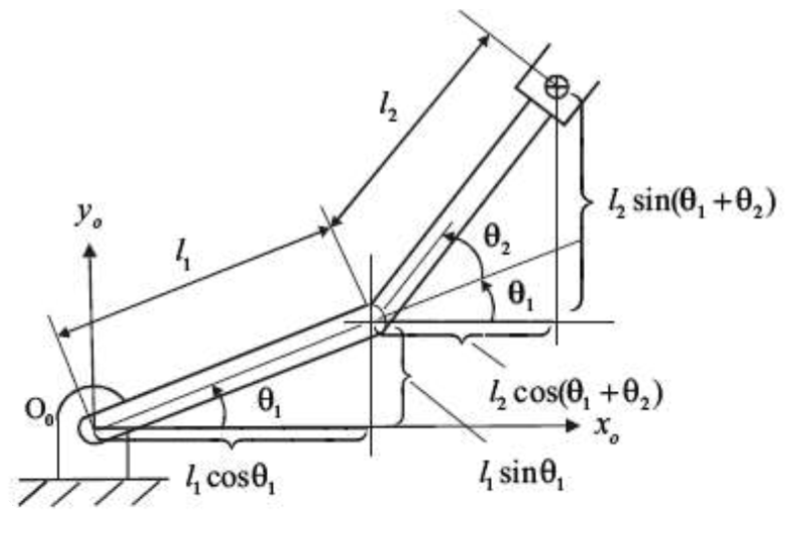
\includegraphics[width=7cm]{./bilder/jacobi-bsp1.png}
\end{minipage}

\begin{minipage}{14cm}
    \vspace{0.5cm}	
    \paragraph{Beispiel 2: }Dreiachsiger Planarroboter: \\
    $
    \begin{bmatrix} 
    x_E \\
    Y_E \\                             
    \end{bmatrix}
    =
    \begin{bmatrix} 
    l_1\cdot cos(\theta_1) + l_2 \cdot cos(\theta_1 + \theta_2) + l_3\cdot cos(\theta_1 + \theta_2 + \theta_3)\\
    l_1\cdot sin(\theta_1) + l_2 \cdot sin(\theta_1 + \theta_2) + l_3\cdot sin(\theta_1 + \theta_2 + \theta_3)\\                     
    \end{bmatrix} \newline
    \null \qquad \gamma = \theta_1 + \theta_2 + \theta_3
    $ \\ \\
    $ J = 
    \begin{bmatrix} 
    \frac{\partial{x_{e}}}{\partial{\theta_{1}}} & 
    \frac{\partial{x_{e}}}{\partial{d_{2}}} & 
    \frac{\partial{x_{e}}}{\partial{\theta_{3}}} \\
    \frac{\partial{y_{e}}}{\partial{\theta_{1}}} & 
    \frac{\partial{y_{e}}}{\partial{d_{2}}} & 
    \frac{\partial{y_{e}}}{\partial{\theta_{3}}} \\
    \frac{\partial{\Phi_{e}}}{\partial{\theta_{1}}} & 
    \frac{\partial{\Phi_{e}}}{\partial{d_{2}}} & 
    \frac{\partial{\Phi_{e}}}{\partial{\theta_{3}}} \\ 
    \end{bmatrix}
    =
    \begin{bmatrix} 
    -l_1 \cdot s_1 -l_2 \cdot s_{12} -l_3\cdot s_{123} & -l_2\cdot s_{12} -l_3\cdot s_{123} & -l_3\cdot s_{123}\\
    l_1\cdot c_1 +l_2\cdot c_{12} +l_3\cdot c_{123} & l_2\cdot c_{12} + l_3\cdot c_{123} & l_3\cdot c_{123}\\
    1 & 1 & 1\\
    \end{bmatrix}
    \\
    \dot{X}
    =
    \begin{bmatrix} 
    \dot{p}_x \\
    \dot{p}_y \\                             
    \end{bmatrix}
    =
    J(q) \cdot         
    \begin{bmatrix} 
    \dot{\theta}_1 \\
    \dot{\theta}_2 \\                             
    \end{bmatrix}$
\end{minipage}
\begin{minipage}{7cm}
    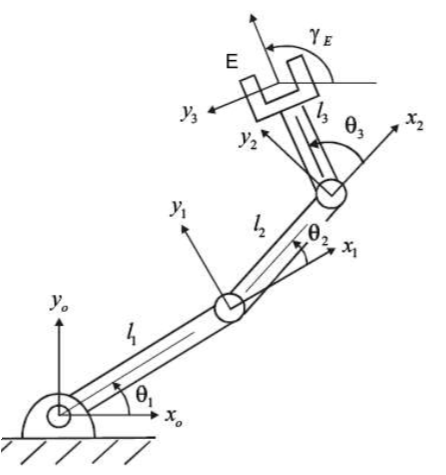
\includegraphics[width=5cm]{./bilder/jacobi-bsp2.png}
\end{minipage}

\clearpage
\subsubsection{Rückwertskinematik}
\begin{tabular}{lll}
    \textbf{Geg}&Geschwindigkeiten des Endeffektors&$\dot{X}$\\
    \textbf{Ges}&Geschwindigkeit der Gelenke&$\dot{q}$\\
\end{tabular}\newline
\textbf{Lösung}: inverse Jacobi-Matrix $ \Longrightarrow \dot{q}=J(q)^{-1}\cdot \dot{x}$ \\
\null\qquad\qquad Nur möglich, wenn J invertierbar ist. (Det $\neq$ 0)

%\paragraph{Beispiel 3: }zweiachsiger Planarroboter: \\
%$J^{-1}=\frac{1}{det(J)}\cdot
%\begin{bmatrix}
%    l_2\cdot c_{12} & l_2 \cdot s_{12}\\
%    -l_1\cdot c_1 - l_2\cdot c_{12} & -l1\cdot s_1 -l_2\cdot s_{12}
%\end{bmatrix}
%$
\subsubsection{Singularität}
Die Jacobi-Matrix kann in singulären Stellungen
nicht invertiert werden (d.h. die Determinante von J ist 0) und der Roboter
kann in bestimmten Richtungen keine Bewegungen
vornehmen. \\
In der Nähe von Singularitäten könnnen die Achsengeschwindigkeiten extrem ansteigen.
%Mehr: Skript-Kinematik (S.11 ff) \& UB5 Bahnplanung (Aufg. 2))
\begin{multicols}{2}
\paragraph{Beispiel 3.1} Singularitätsbestimmung eines zweiachsigen Planarroboters\newline
\null\hspace{0.5cm}\begin{tabular}{ll}
    \textbf{Gegeben:}& Jacobi-Matrix\\
    \textbf{Gesucht:}& Singularität\\
    \textbf{Vorgehen:} & det(J)= 0 setzen\\
\end{tabular}
\paragraph{Beispiel 3.2} Geschwindigeit in singulärer Stellung\newline
\null\hspace{0.5cm}\begin{tabular}{ll}
    \textbf{Gegeben:}& Jacobi-Matrix\\
    \textbf{Gesucht:}& Geschwindigeit\\
    \textbf{Formel:} & $ \dot{\theta}= J^{-1}\cdot \dot{x}$\\
    \textbf{Vorgehen:} & det(J) $\rightarrow$ 0 \\
\end{tabular}
\end{multicols}
\subsection{Roboterstatik}
Momente, welche an den Achsgelenken wirken:\newline
$\tau_{n}={}^0J^T_n \cdot {}^0F_n$  \\
Externe Momente / Kräfte, welche am n-ten Glied wirken:\newline
${}^0F_n = \begin{bmatrix} {}^0F_{x,n} & {}^0F_{y,n} & {}^0F_{z,n} & {}^0M_{x,n}
& {}^0M_{y,n} & {}^0M_{z,n}
\end{bmatrix}^{T} $ \newline
\paragraph{Beispiel 4} Kräfte eines zweichasigen Planarroboter\newline
Der Roboter soll mit dem globalen Kraftvektor ${}^0F$ gegen einen fixen Körper drücken.\newline
\null\hspace{0.5cm}\begin{tabular}{ll}
    \textbf{Gegeben:}& Jacobi-Matrix\\
    \textbf{Gesucht:}& erforderliches Antriebsmoment $\tau_1$ und $\tau_2$\\
    \textbf{Vorgehen:} & $\tau_{n}={}^0J^T_n \cdot {}^0F_n$  \\
\end{tabular}$\null \qquad\qquad
\begin{bmatrix}
\tau_{1} \\ \tau_{2} \\ \tau_{3}
\end{bmatrix}          
=  J \cdot
\begin{bmatrix}
F_{x} \\ F_{y} \\ F_{z}
\end{bmatrix}
$
\clearpage

